\documentclass[acmsmall, screen, review, nonacm]{acmart}

\usepackage{listings}
\usepackage{tikz}
\usepackage{multirow}
\usepackage{array}
\usetikzlibrary{arrows,decorations.pathmorphing,backgrounds,positioning,fit,shapes,matrix}
\newcommand{\JastAdd}{\textsc{Jast\-Add}}
\newcommand{\ExtendJ}{\textsc{ExtendJ}}
\newcommand{\IntraJ}{\textsc{IntraJ}}
\newcommand{\CAT}{\textsc{CAT}}
\newcommand{\eval}[2]{\textsc{#1}$_{\color{gray!70}{\pm#2}}$}
\newcommand{\basicStacked}{\textsc{Basic\-Stacked}}
\newcommand{\relaxedMonolithic}{\textsc{Relaxed\-Monolithic}}
\newcommand{\relaxedstacked}{\textsc{Relaxed\-Stacked}}
\newcommand{\relmon}{\textsc{rm}} %Abbreviation for relaxed Monolithic
\newcommand{\relstk}{\textsc{rs}} %Abbreviation for relaxed stacked
\newcommand{\code}[1]{\texttt{#1}}
\newcommand{\slowdown}[1]{$-$ #1 \color{red}{$\downarrow$}}
\newcommand{\speedup}[1]{$+$ #1 \color{teal}{$\uparrow$}}
\newcommand{\slowdownnew}[1]{$\times$ #1 \color{red}{$\downarrow$}}
\newcommand{\speedupnew}[1]{$\times$ #1 \color{teal}{$\uparrow$}}
\newcommand{\evaltimeout}[1]{%
    $\geq$ \textsc{#1}~\raisebox{-0.2\height}{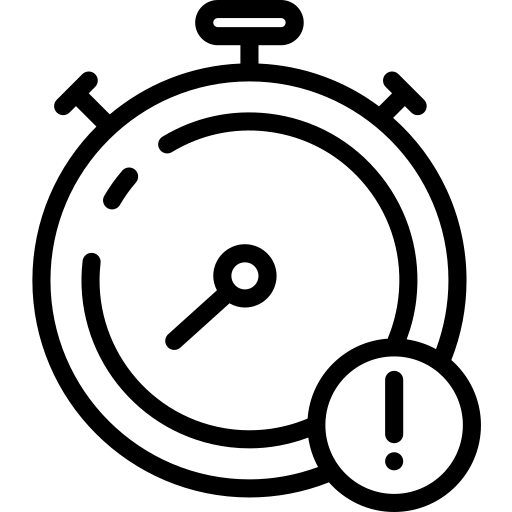
\includegraphics[height=1em]{timeout.png}}%
}
\newcommand{\gespeedup}[1]{$\geq$ #1 \color{teal}{$\uparrow$}}
\newcommand{\same}{\color{gray}{$\approx$}}

\newcommand{\extendjbaseline}{\ExtendJ$_{\relmon}$}
\newcommand{\extendjrelaxed}{\ExtendJ$_{\relstk}$}



\newcommand{\intrajbaseline}{\IntraJ$_{\relmon}$}
\newcommand{\intrajrelaxed}{\IntraJ$_{\relstk}$}


\newcommand{\percentwrt}[1]{\footnotesize
$\Delta$\%$^{\scriptscriptstyle\text{w.r.t}}_{\scriptscriptstyle\text{#1}}$%
}











\lstset{basicstyle=\scriptsize\ttfamily,
        escapeinside={/+}{+/},
        keywordstyle=[1]\bfseries}



\AtBeginDocument{%
  \providecommand\BibTeX{{%
    Bib\TeX}}}

%% Rights management information.  This information is sent to you
%% when you complete the rights form.  These commands have SAMPLE
%% values in them; it is your responsibility as an author to replace
%% the commands and values with those provided to you when you
%% complete the rights form.
\setcopyright{acmcopyright}
\copyrightyear{2018}
\acmYear{2018}
\acmDOI{XXXXXXX.XXXXXXX}

%% These commands are for a PROCEEDINGS abstract or paper.
\acmConference[PLDI]{}{October 20-25,
  2024}{Pasadena, USA}


\acmPrice{15.00}
\acmISBN{978-1-4503-XXXX-X/18/06}




\begin{document}



\title{Artifact Evaluation Results}
\subtitle{Efficient Demand Evaluation of Fixed-Point Attributes Using Static Analysis}


\author{Idriss Riouak}
\email{idriss.riouak@cs.lth.se}
\orcid{0000-0003-3520-2262}
\author{Niklas Fors}
\email{niklas.fors@cs.lth.se}
\orcid{0000-0003-2714-9457}
\affiliation{%
  \institution{Lund University}
  \streetaddress{Ole R\"{o}mers v\"{a}g 3}
  \city{Lund}
  \country{Sweden}
  \postcode{22363}
}

\author{Jesper {\"O}qvist}
\email{jesper.oqvist@cognibotics.com }
\affiliation{%
  \institution{Cognibotics AB}
  \streetaddress{Scheelevägen 15}
  \city{Lund}
  \country{Sweden}
  \postcode{22370}
}
\orcid{0000-0001-5453-3695}
\author{G{\"o}rel Hedin}
\email{gorel.hedin@cs.lth.se}
\orcid{0000-0002-3003-2623}
\author{Christoph Reichenbach}
\email{chirstoph.reichenbach@cs.lth.se}
\orcid{0000-0003-0608-7023}
\affiliation{%
  \institution{Lund University}
  \streetaddress{Ole R\"{o}mers v\"{a}g 3}
  \city{Lund}
  \country{Sweden}
  \postcode{22363}
}



\renewcommand{\shortauthors}{Riouak et al.}


\maketitle

This document presents the results of our artifact evaluation. Each section
includes data generated from executing our artifact. The data is presented in
tables and figures with references to the corresponding sections in the paper.

\section{Case Study: LL(1) Parser Construction}
This section presents the results of the LL(1) Parser Construction case study.
This case study corresponds to Section~5.2 in the paper.


\begin{table}[H]
    \setlength{\tabcolsep}{2pt} 
    \begin{tabular}{|l|c|c|c|c|c|c|}
        \hline
        \textsc{Language} & \textbf{\#T} & \textbf{\#P} & \textbf{Old Stacked} &\textbf{Basic Stacked} & \textbf{Relaxed Monolithic} & \textbf{Relaxed Stacked} \\ \cline{2-5}
        \hline
        \textsc{Java 1.2}    & 155 & 332 & \eval{9.21}{0.31} &   \eval{7.52}{0.16}           &      \eval{16.26}{0.47}              &    \eval{7.86}{0.26}   \\ \hline
    \end{tabular}
    \caption{Startup performance results for the \textsc{Java 1.2 grammar} benchmark. Includes the number of terminals (\#T) and productions (\#P). The measurements are reported in milliseconds. }
    \label{tab:cfg}
\end{table}




\section{Case Study: \textsc{IntraJ}}
This section presents the results of the \textsc{IntraJ} case study.
This case study corresponds to Section~5.4 in the paper.


\subsection{Dead Assignment Analysis (DAA)}
Table~\ref{tab:daa} presents the results of the Null-pointer Exception Analysis, corresponding to the right portion of Table~3 in the referenced paper.

\input{intraj-table-daa.tex}




\subsection{Null-pointer Exception Analysis (NPA)}
Table~\ref{tab:npa} presents the results of the Null-pointer Exception Analysis, corresponding to the left portion of Table~3 in the referenced paper.
\input{intraj-table-npa.tex}




\section{On-Demand Analysis}
This section presents a comparative analysis of \IntraJ{}'s steady-state execution time.
The figures show the average execution time for both Dead Assignment Analysis and Null-pointer Exception Analysis.
The analysis is conducted on 10, 20, 50, 100, and 200 methods randomly selected from each analysed benchmark.
\begin{figure}[H]
  \centering
  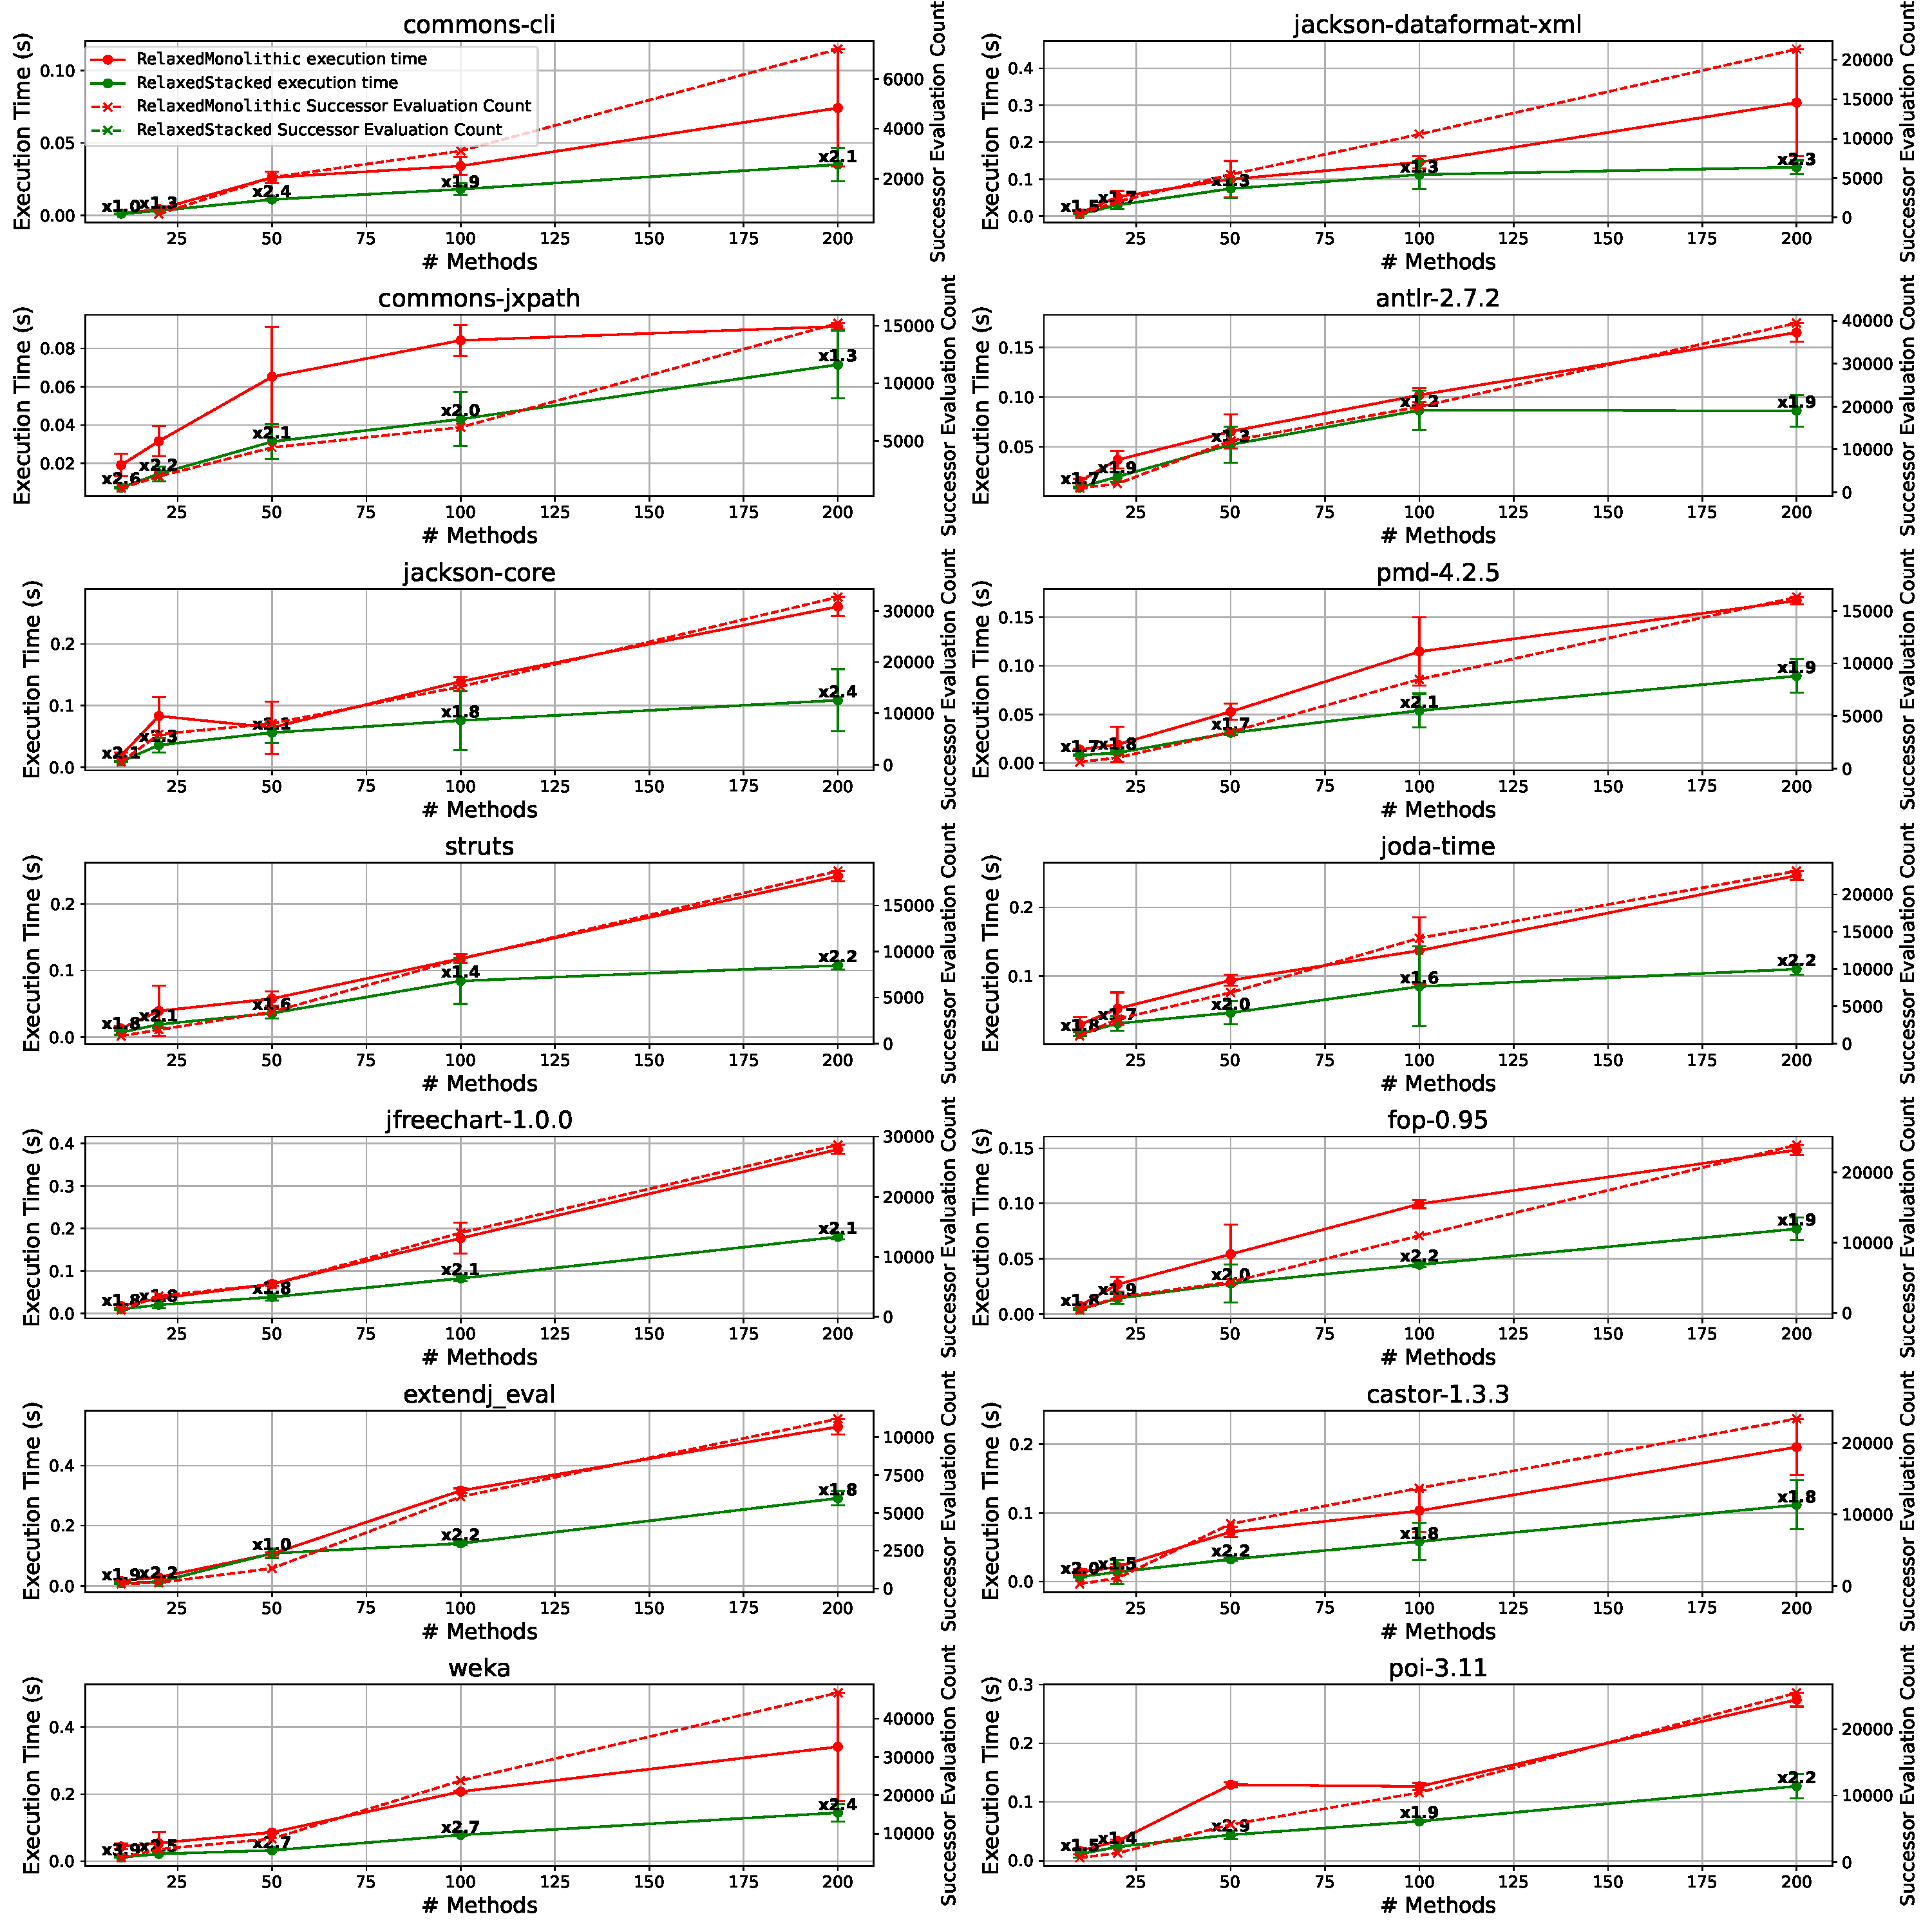
\includegraphics[width=0.9\textwidth]{intraj_ondemand_daa_relaxedmonolithic_vs_intraj_ondemand_daa_relaxedstackedon-demand.pdf}
  \caption{
    Steady-state performance of running dead assignment (left) and null-pointer dereference analysis (right) for randomly selected sets of methods. Solid lines represent execution time (left axis, seconds). Dashed lines represent successor attribute evaluations (right axis, count). Red lines represent RelaxedMonolithic, green lines RelaxedStacked.
  }
\end{figure}

\begin{figure}[H]
  \centering
  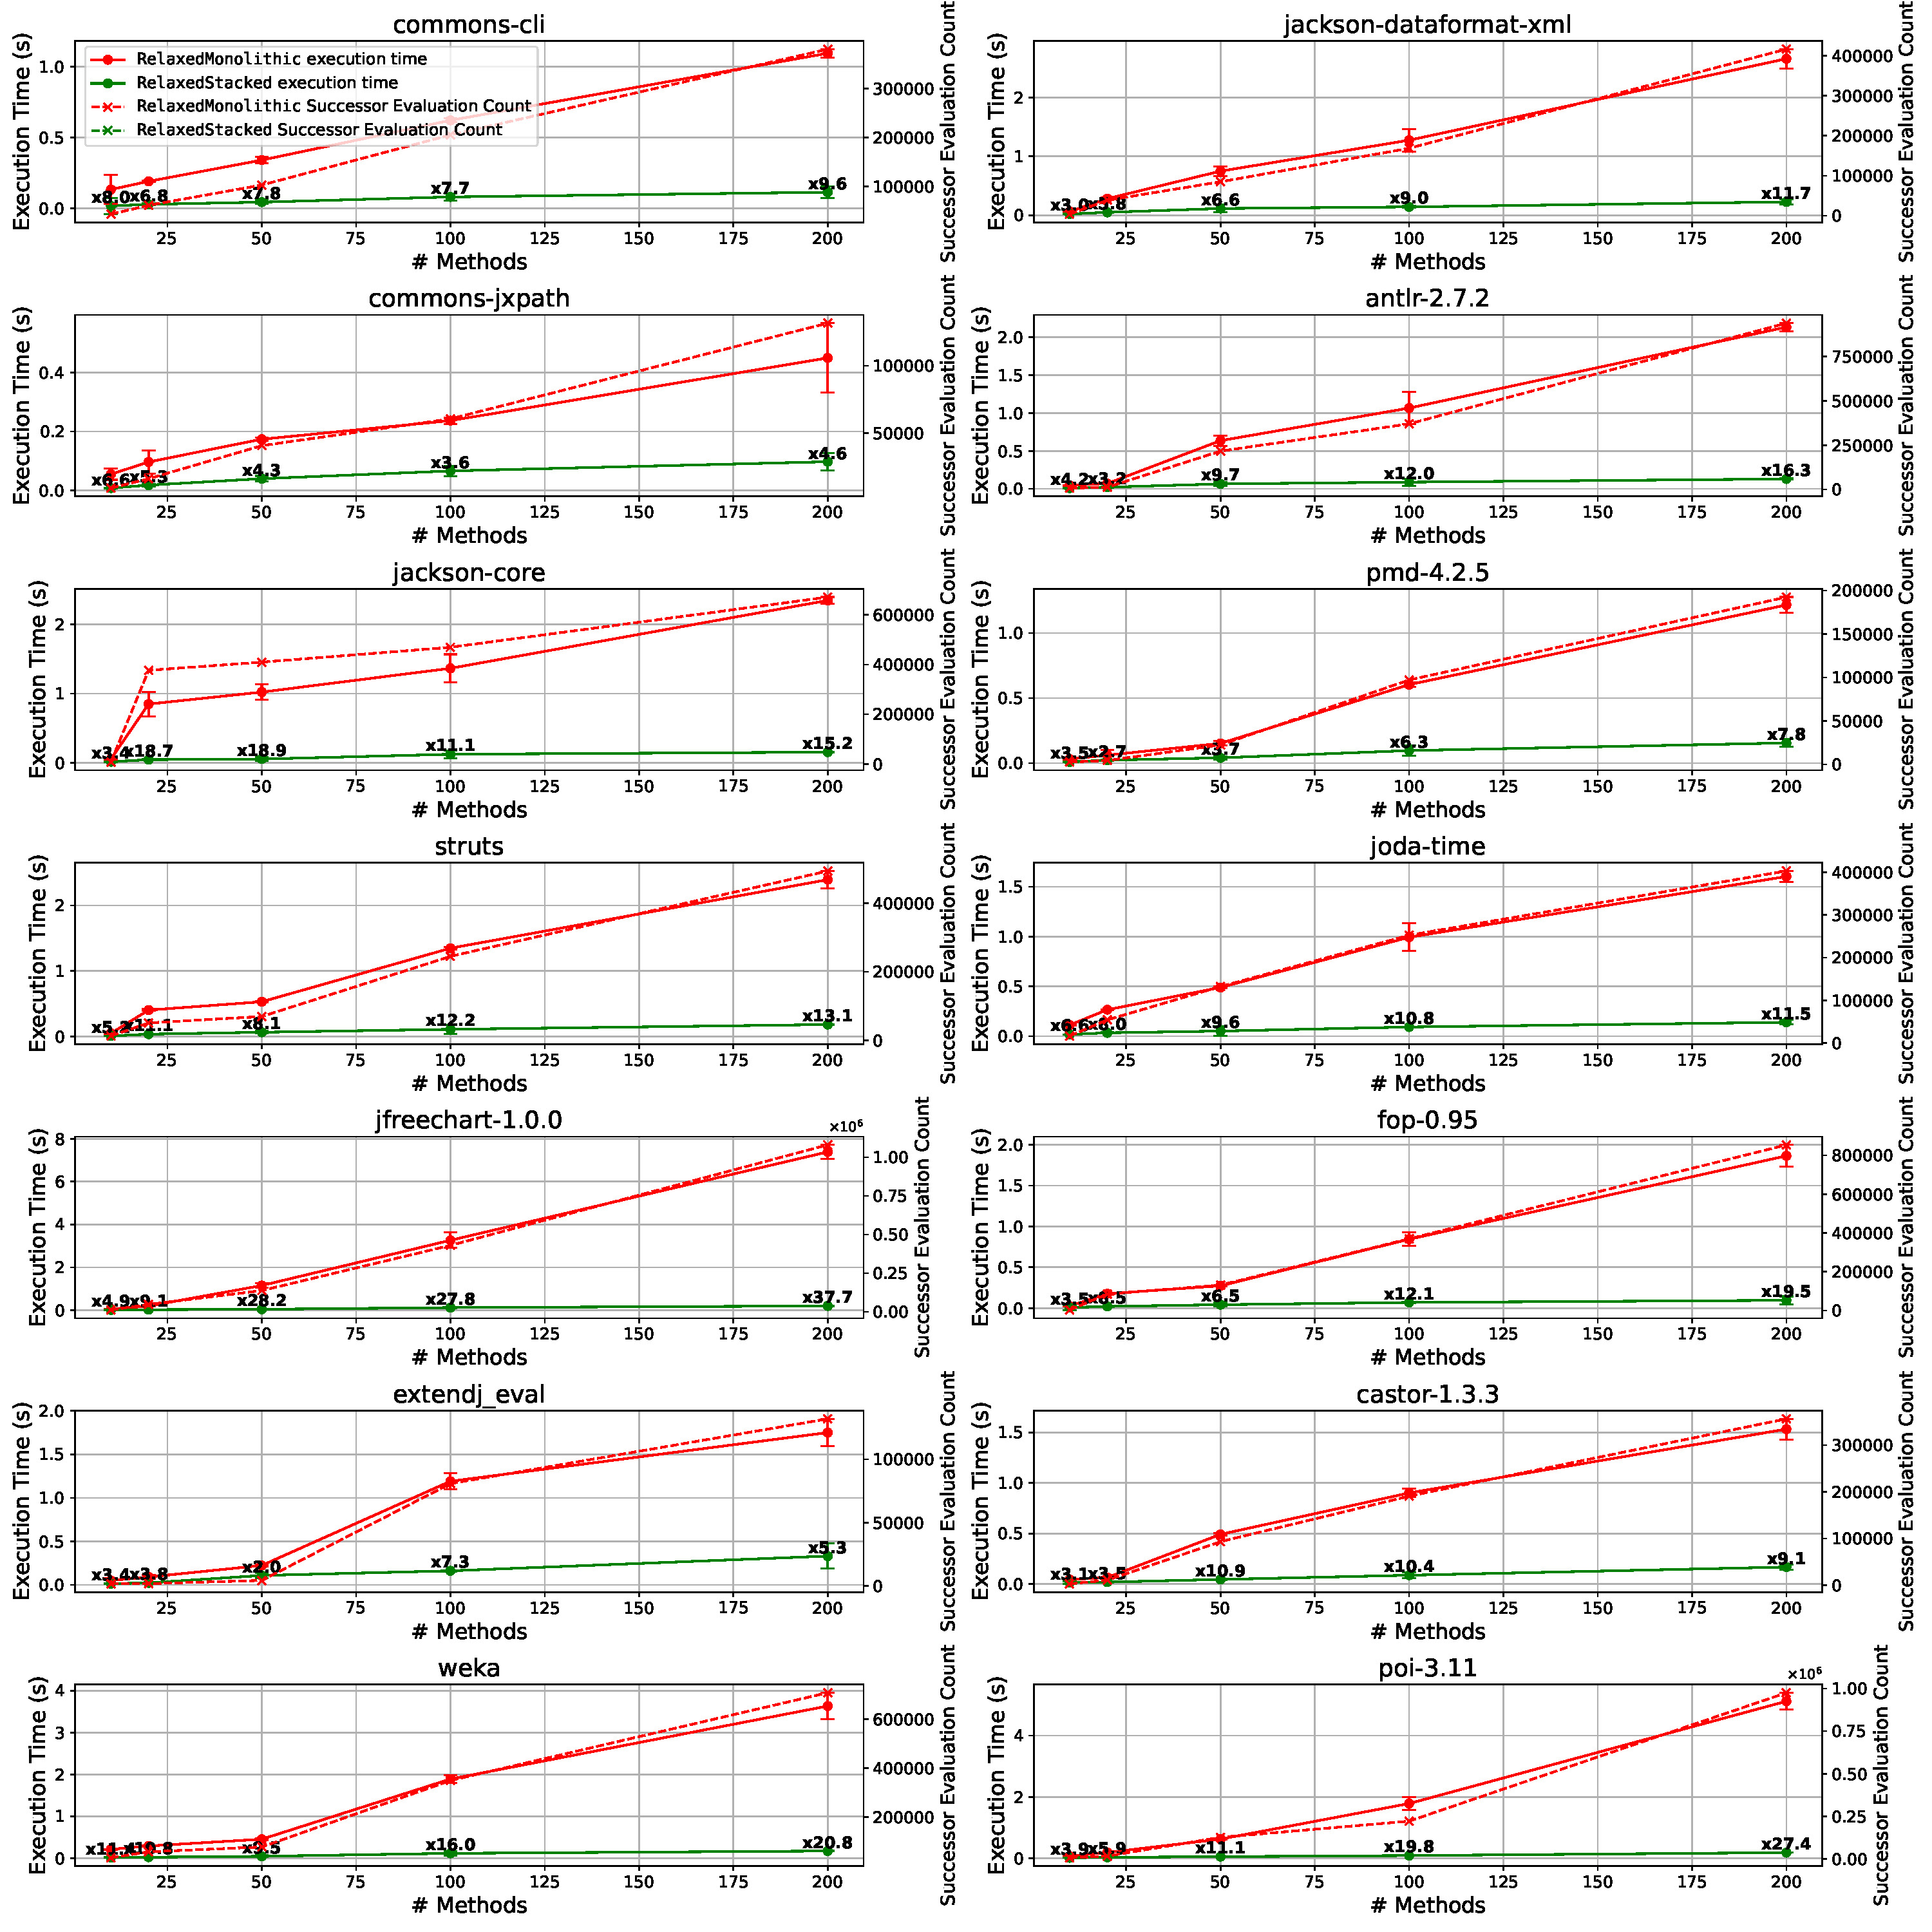
\includegraphics[width=0.9\textwidth]{intraj_ondemand_npa_relaxedmonolithic_vs_intraj_ondemand_npa_relaxedstackedon-demand.pdf}
  \caption{
    Steady-state performance of running dead assignment (left) and null-pointer dereference analysis (right) for randomly selected sets of methods. Solid lines represent execution time (left axis, seconds). Dashed lines represent successor attribute evaluations (right axis, count). Red lines represent RelaxedMonolithic, green lines RelaxedStacked.
  }
\end{figure}

\appendix
\section{Case Study: \textsc{ExtendJ}}
This section presents the results of the \textsc{ExtendJ} case study, which
correspond to Appendix B of the paper. Table~\ref{tab:extendj} provides the
performance results for the \ExtendJ{} compiler, illustrating both startup and
steady-state performance for \relaxedMonolithic{} and \relaxedstacked{}
configurations. Table~\ref{tab:extendj} aligns with Table~4 in the
paper.


\begin{table}[H]
	\begin{tabular}{|l|rrr|rrr|}
	\hline
	\multirow{3}{*}{\textsc{Benchmark}} & \multicolumn{3}{c|}{\textsc{Start up}} & \multicolumn{3}{c|}{\textsc{Steady State}} \\ \cline{2-7}
	& \multicolumn{1}{c|}{\textsc{Relaxed-}} & \multicolumn{2}{c|}{\textsc{Relaxed-}} & \multicolumn{1}{c|}{\textsc{Relaxed-}} & \multicolumn{2}{c|}{\textsc{Relaxed-}} \\
	& \multicolumn{1}{c|}{\textsc{Monolithic}} & \multicolumn{2}{c|}{\textsc{Stacked}} & \multicolumn{1}{c|}{\textsc{Monolithic}} & \multicolumn{2}{c|}{\textsc{Stacked}} \\ \cline{2-7}
	& \multicolumn{1}{c|}{Time (s)} & \multicolumn{1}{c|}{Time (s)} & \textsc{Speedup} & \multicolumn{1}{c|}{Time (s)} & \multicolumn{1}{c|}{Time (s)} & \textsc{Speedup} \\ \hline
	 \code{commons-cli} & \multicolumn{1}{r|}{\eval{1.01}{0.04}} & \multicolumn{1}{r|}{\eval{1.01}{0.14}} & \same{} & \multicolumn{1}{r|}{\eval{0.23}{0.01}} & \multicolumn{1}{r|}{\eval{0.24}{0.02}} & \same{} \\ \hline
	 \code{jackson-dataformat-xml} & \multicolumn{1}{r|}{\eval{2.41}{0.20}} & \multicolumn{1}{r|}{\eval{2.39}{0.64}} & \same{} & \multicolumn{1}{r|}{\eval{0.69}{0.10}} & \multicolumn{1}{r|}{\eval{0.68}{0.01}} & \same{} \\ \hline
	 \code{commons-jxpath} & \multicolumn{1}{r|}{\eval{1.74}{0.22}} & \multicolumn{1}{r|}{\eval{1.73}{0.22}} & \same{} & \multicolumn{1}{r|}{\eval{0.44}{0.01}} & \multicolumn{1}{r|}{\eval{0.44}{0.12}} & \same{} \\ \hline
	 \code{antlr-2.7.2} & \multicolumn{1}{r|}{\eval{1.94}{0.23}} & \multicolumn{1}{r|}{\eval{2.01}{0.13}} & \slowdownnew{0.96} & \multicolumn{1}{r|}{\eval{0.63}{0.13}} & \multicolumn{1}{r|}{\eval{0.60}{0.05}} & \speedupnew{1.05} \\ \hline
	 \code{jackson-core} & \multicolumn{1}{r|}{\eval{3.51}{0.22}} & \multicolumn{1}{r|}{\eval{3.36}{0.16}} & \speedupnew{1.04} & \multicolumn{1}{r|}{\eval{1.06}{0.15}} & \multicolumn{1}{r|}{\eval{1.08}{0.18}} & \same{} \\ \hline
	 \code{pmd-4.2.5} & \multicolumn{1}{r|}{\eval{4.47}{0.21}} & \multicolumn{1}{r|}{\eval{4.47}{0.26}} & \same{} & \multicolumn{1}{r|}{\eval{1.48}{0.10}} & \multicolumn{1}{r|}{\eval{1.47}{0.02}} & \same{} \\ \hline
	 \code{struts} & \multicolumn{1}{r|}{\eval{6.03}{0.36}} & \multicolumn{1}{r|}{\eval{5.88}{0.52}} & \speedupnew{1.03} & \multicolumn{1}{r|}{\eval{2.26}{0.34}} & \multicolumn{1}{r|}{\eval{2.22}{0.06}} & \same{} \\ \hline
	 \code{joda-time} & \multicolumn{1}{r|}{\eval{5.35}{0.40}} & \multicolumn{1}{r|}{\eval{5.09}{0.42}} & \speedupnew{1.05} & \multicolumn{1}{r|}{\eval{2.20}{0.29}} & \multicolumn{1}{r|}{\eval{2.18}{0.02}} & \same{} \\ \hline
	 \code{jfreechart-1.0.0} & \multicolumn{1}{r|}{\eval{4.53}{0.32}} & \multicolumn{1}{r|}{\eval{4.68}{0.22}} & \slowdownnew{0.97} & \multicolumn{1}{r|}{\eval{1.97}{0.14}} & \multicolumn{1}{r|}{\eval{1.98}{0.16}} & \same{} \\ \hline
	 \code{fop-0.95} & \multicolumn{1}{r|}{\eval{5.72}{0.30}} & \multicolumn{1}{r|}{\eval{5.69}{0.45}} & \same{} & \multicolumn{1}{r|}{\eval{2.28}{0.14}} & \multicolumn{1}{r|}{\eval{2.29}{0.19}} & \same{} \\ \hline
	 \code{extendj\_eval} & \multicolumn{1}{r|}{\eval{7.24}{0.53}} & \multicolumn{1}{r|}{\eval{7.26}{0.69}} & \same{} & \multicolumn{1}{r|}{\eval{4.53}{0.32}} & \multicolumn{1}{r|}{\eval{4.40}{0.43}} & \speedupnew{1.03} \\ \hline
	 \code{castor-1.3.3} & \multicolumn{1}{r|}{\eval{7.58}{0.25}} & \multicolumn{1}{r|}{\eval{7.59}{0.40}} & \same{} & \multicolumn{1}{r|}{\eval{3.87}{0.12}} & \multicolumn{1}{r|}{\eval{3.91}{0.17}} & \same{} \\ \hline
	 \code{weka} & \multicolumn{1}{r|}{\eval{11.49}{0.56}} & \multicolumn{1}{r|}{\eval{11.38}{0.55}} & \same{} & \multicolumn{1}{r|}{\eval{6.25}{0.26}} & \multicolumn{1}{r|}{\eval{6.15}{0.35}} & \same{} \\ \hline
	 \code{poi-3.11} & \multicolumn{1}{r|}{\eval{16.23}{0.70}} & \multicolumn{1}{r|}{\eval{16.21}{1.06}} & \same{} & \multicolumn{1}{r|}{\eval{9.12}{0.35}} & \multicolumn{1}{r|}{\eval{9.20}{0.42}} & \same{} \\ \hline
	\end{tabular}
    \caption{\label{tab:extendj} Performance comparison of ExtendJ’s execution time during startup and steady state.}
    
\end{table}

\end{document}
\endinput
